\documentclass[twoside]{article}

\usepackage[preprint]{aistats2027}
\usepackage[round,authoryear]{natbib}
\usepackage{amsmath,amssymb,amsthm}
\usepackage{booktabs}
\usepackage{graphicx}
\usepackage{microtype}
\usepackage{xcolor}
\usepackage{balance}
\usepackage{url}

\renewcommand{\bibname}{References}
\renewcommand{\bibsection}{\subsubsection*{\bibname}}
\bibliographystyle{apalike}

\newtheorem{theorem}{Theorem}
\newtheorem{proposition}{Proposition}
\newtheorem{corollary}{Corollary}
\newcommand{\E}{\mathbb E}
\newcommand{\Pcal}{\mathcal P}
\newcommand{\TV}{\operatorname{TV}}
\newcommand{\diam}{\operatorname{diam}}

\begin{document}
\runningtitle{Sharp Limits for Pass@k Forecasting}
\runningauthor{}

\twocolumn[
\aistatstitle{Extrapolation Is an Assumption:\\Sharp Limits for Pass@k Forecasting}

\aistatsauthor{Pahan Dewasurendra}

\aistatsaddress{Johns Hopkins University\\[4pt] July 24, 2026}
]

\begin{abstract}
Repeated sampling can reveal capabilities and risks that are invisible in one language-model attempt, motivating forecasts of pass@\(k\) from much smaller response banks. We ask what such data support without a parametric law for task difficulty. With \(b\) attempts per task, the count distribution identifies exactly the first \(b\) moments of the latent success-probability distribution. We prove that the worst-case diameter of pass@\(k\)'s identified set is exactly twice the best degree-\(b\) uniform approximation error for \(x^k\). A theorem of Newman and Rivlin then yields explicit binomial-tail bounds and a sharp extrapolation transition at \(k\asymp b^2\). We extend the limit to finite task sets through a Hellinger modulus and to adaptive policies with a per-task cap. We also give two finite-sample confidence intervals: a global polynomial interval that attains the limiting worst-case diameter and a data-adaptive projection interval. At 128 tasks and 78 attempts per task, any honest 95\% interval for population pass has expected-length lower bounds \(0.276\) and \(0.686\) for pass@1000 and pass@10000. In synthetic audits, narrow taskwise Beta intervals have zero coverage under seven nonparametric alternatives. Across 22 public response banks, model-free intervals include every 10,000-response reference but are necessarily wide at distant horizons. Pass@\(k\) extrapolation can be useful, but its uncertainty must disclose the structural assumptions that make it possible.
\end{abstract}

\section{Introduction}

Repeated inference is now a practical scaling axis for language models. Large response banks show substantial gains from trying a task many times \citep{brown2024}. The aggregate pass@\(k\) curve is also used to forecast capability and safety at budgets far beyond those directly sampled. Recent methods fit heavy-tailed task-difficulty laws \citep{schaeffer2025}, use a population Beta-binomial model and adaptive allocation \citep{kazdan2025}, or place independent Beta posteriors on tasks \citep{tailpass2026,hariri2026}. These approaches answer an important conditional question: what does pass@\(k\) look like if the chosen structural model extrapolates correctly? Related scaling theories derive power-law curves from Beta or regularly varying latent difficulty models \citep{levi2025,levi2026}.

We study the complementary question: what is learned before that assumption? For a task with one-attempt success probability \(P\), the target is
\begin{equation}
 \theta_k(F)=\E_F[1-(1-P)^k],
\label{eq:target}
\end{equation}
where \(F\) is the population distribution of \(P\). We observe \(b\) independent attempts per task. This is a classical binomial-mixture model. It is also the incidence model underlying species-accumulation curves \citep{colwell2004}. Our contribution is not a new mixture representation. It is a sharp account of the information boundary for the pass@\(k\) functional, together with finite-task inference and an audit of current forecasting practice.

The boundary is governed by polynomial approximation. The complete count histogram identifies all polynomials of degree at most \(b\). Consequently, two task populations are observationally equivalent exactly when they agree on the first \(b\) moments. We show that the largest possible pass@\(k\) gap between such populations is \[ D_{b,k}=2\inf_{q\in\Pcal_b}\|x^k-q(x)\|_{\infty,[0,1]}. \] This equality turns a 1976 approximation theorem \citep{newman1976} into explicit limits for pass@\(k\). If \(H\sim\operatorname{Binomial}(2k,1/2)\), then \[ \frac{\Pr(|H-k|>b)}{2e} \leq D_{b,k}\leq 2\Pr(|H-k|>b). \] Thus model-free extrapolation is accurate uniformly over task populations when \(k\ll b^2\), and can be highly ambiguous when \(k\) reaches or exceeds that scale.

Our main contributions are:
\begin{itemize}
\item We characterize the sharp identified set for each observable count law
by moment duality, and prove the exact worst-case diameter above.
\item We derive confidence-set lower bounds that persist with infinitely many
tasks, a finite-task Hellinger modulus, and an indistinguishability extension to adaptive sampling with a deterministic per-task cap.
\item We construct global and data-adaptive finite-sample confidence
intervals. The global interval is honest for heterogeneous fixed tasks and is asymptotically sharp in worst-case width.
\item We test the limits against current methods. A numerically moment-matched
pair has count probabilities equal within \(1.7\times10^{-12}\) at \(b=8\), but pass@1000 values \(0.167\) and \(0.950\). In 3,200 synthetic datasets, taskwise Beta intervals are well calibrated only under their model-correct case. A 59,400-forecast audit on 22 public response banks finds increasing point error and intervals whose narrowness does not reflect nonparametric ambiguity.
\end{itemize}

The result is not that all extrapolation should stop at \(b\). Structure can be scientifically justified and empirically useful. Rather, forecasts beyond the identified regime should separate sampling uncertainty from assumptions about the unobserved lower tail of task success probabilities.

\section{Model and Identification}

\paragraph{Observation model.}
For tasks \(i=1,\ldots,M\), let \(P_i\) be iid from an unknown probability law \(F\) on \([0,1]\). Conditional on \(P_i\), \[ S_i\mid P_i\sim\operatorname{Binomial}(b,P_i). \] The population count probabilities are \[ \pi_s(F)=\binom bs\int p^s(1-p)^{b-s}\,dF(p), \qquad s=0,\ldots,b. \] We first study population identification, which corresponds to knowing \(\pi(F)\) exactly. Section~\ref{sec:inference} returns to finite \(M\) and also covers fixed heterogeneous task probabilities.

\begin{proposition}[Observable information]
\label{prop:moments}
The count law \(\pi(F)\) identifies exactly \(\int q(p)dF(p)\) for every \(q\in\Pcal_b\), equivalently the first \(b\) moments of \(F\). Hence \(\theta_k\) is identified for \(k\leq b\), with the usual combinatorial pass@\(k\) estimator, but not generally for \(k>b\).
\end{proposition}

This follows because the \(b+1\) binomial probabilities are expectations of the Bernstein basis, which spans \(\Pcal_b\). Finite-moment identification is well known in binomial mixtures. \citet{basu2026} recently used the same boundary for exact inference on mixing-distribution CDFs and quantiles.

\subsection{Exact identified sets}

Let \(\mu_j=\int p^j dF(p)\), including \(\mu_0=1\), be the moments recovered from \(\pi(F)\). Generalized moment duality gives the exact endpoints
\begin{align}
 L_k(\mu)
 &=\sup_{\substack{q\in\Pcal_b\\q\leq h_k}}
   \sum_{j=0}^b q_j\mu_j,
&
 U_k(\mu)
 &=\inf_{\substack{q\in\Pcal_b\\q\geq h_k}}
   \sum_{j=0}^b q_j\mu_j,
\label{eq:momentdual}
\end{align}
where \(h_k(p)=1-(1-p)^k\) and \(q(p)=\sum_jq_jp^j\). The primal problems optimize \(\int h_kdF\) over all laws with moments \(\mu\). Compact generalized moment problems have no duality gap \citep{deklerk2019,halaseh2026}. A dual optimizer need not exist for boundary moment vectors, so \eqref{eq:momentdual} is stated using a supremum and an infimum. Convexity shows that the identified set is the full interval \([L_k(\mu),U_k(\mu)]\).

The width depends on the observed count law. The following theorem identifies its largest possible value.

\begin{theorem}[Sharp worst-case diameter]
\label{thm:diameter}
Let \[ E_{b,k}=\inf_{q\in\Pcal_b}\|x^k-q(x)\|_{\infty,[0,1]}. \] Then \[ \sup_{\mu}\{U_k(\mu)-L_k(\mu)\}=D_{b,k}=2E_{b,k}. \] Moreover, there are two probability laws attaining this gap while inducing the same complete count distribution.
\end{theorem}

\paragraph{Proof sketch.}
If \(F\) and \(G\) match through degree \(b\), every \(q\in\Pcal_b\) cancels. The target difference is therefore at most \(2\|x^k-q\|_\infty\). For the reverse inequality, quotient-space duality for \(C[0,1]/\Pcal_b\) and the Riesz representation theorem give a signed measure \(\nu\) of total variation one that annihilates \(\Pcal_b\) and integrates \(x^k\) to \(E_{b,k}\). Since \(\nu\) annihilates constants, its positive and negative parts each have mass \(1/2\). Normalizing them yields the required probability laws and gap \(2E_{b,k}\). Full proofs are in the supplement.

\begin{corollary}[Extrapolation horizon]
\label{cor:horizon}
For \(H\sim\operatorname{Binomial}(2k,1/2)\), let \(T_{b,k}=\Pr(|H-k|>b)\). Then \[ \frac{T_{b,k}}{2e}\leq D_{b,k}\leq 2T_{b,k}. \] In particular, the worst-case identification transition is \(b\asymp\sqrt{k}\), or \(k\asymp b^2\).
\end{corollary}

To obtain the corollary, map approximation of \(x^k\) on \([0,1]\) by degree \(b\) polynomials to approximation of \(x^{2k}\) on \([-1,1]\) by degree \(2b\) polynomials. \citet{newman1976} bound that error between \(T_{b,k}/(4e)\) and \(T_{b,k}\). The \(b^2\) approximation transition is theirs. Its interpretation as the exact pass@\(k\) ambiguity is new here.

\begin{corollary}[What a probability floor buys]
\label{cor:floor}
Restrict both task populations to \(P\in[p_0,1]\), for a declared \(p_0\in[0,1]\). The sharp worst-case diameter becomes \[ D_{b,k}(p_0)=(1-p_0)^kD_{b,k}. \]
\end{corollary}

Set \(x=1-p\) and rescale \(x=(1-p_0)y\). Degree-\(b\) moment matching and polynomial approximation are preserved, while the target monomial is multiplied by \((1-p_0)^k\). This quantifies the value and the risk of a lower tail assumption. At \(b=78,k=10000\), the unrestricted diameter is \(0.285\). A known floor \(p_0=10^{-4}\) reduces it to \(0.105\), while \(p_0=10^{-3}\) reduces it below \(1.3\times10^{-5}\). Such a floor can make distant forecasts precise, but it rules out impossible and extremely hard tasks. With finitely many attempts, its validity comes from domain knowledge, not from seeing no success on a task.

\begin{figure}[t]
\centering
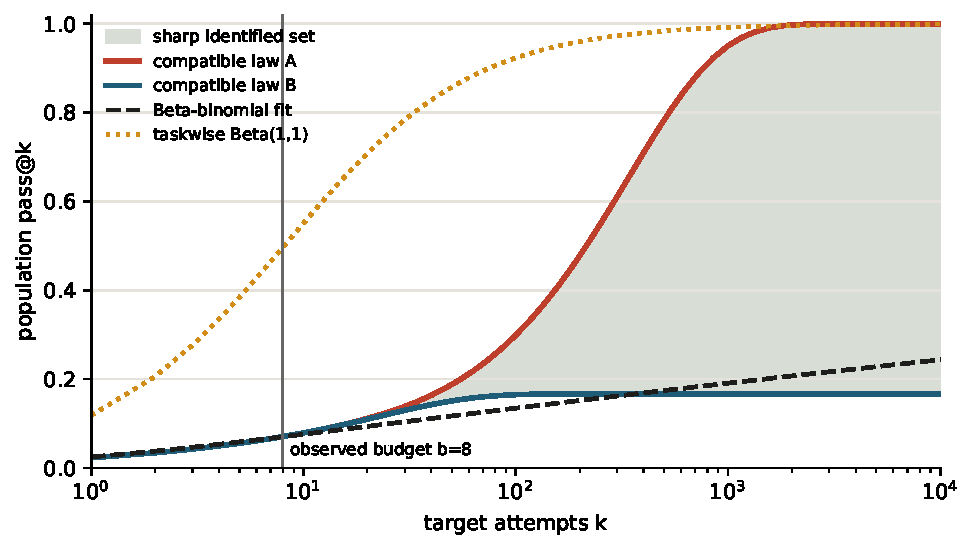
\includegraphics[width=\columnwidth]{matched_pair_curves.pdf}
\caption{Two task populations induce the same count law for \(b=8\) but
diverge after the observed budget. The shaded region is the sharp identified set for their shared moments. Parametric fits select narrow trajectories inside it.}
\label{fig:pair}
\end{figure}

\paragraph{A sharp ambiguity example.}
Figure~\ref{fig:pair} numerically constructs the dual extremizers at \(b=8\). Each is supported on five probabilities. Their induced count probabilities differ by at most \(1.7\times10^{-12}\), while pass@1000 is \(0.16689\) under one and \(0.95019\) under the other. The resulting diameter \(0.78330\) agrees with \(2E_{8,1000}\) to \(10^{-11}\). The same calculation gives approximate diameters \(0.509\) at \(b=16,k=1000\), \(0.707\) at \(b=32,k=10000\), and \(0.389\) at \(b=64,k=10000\).

\section{Honest Inference}
\label{sec:inference}

Identification ambiguity does not vanish as the number of tasks grows. It is also not the only obstacle at finite \(M\).

\begin{theorem}[Confidence-set limits]
\label{thm:ci-lower}
Let \(C\) have coverage at least \(1-\alpha\) under two task-population laws \(F,G\). If they induce identical count laws and have target gap \(\Delta\), then
\begin{align*}
 \Pr\{\diam(C)\geq\Delta\}&\geq1-2\alpha,\\
 \E[\diam(C)]&\geq(1-2\alpha)\Delta.
\end{align*}
More generally, write \(q_F,q_G\) for their one-task count laws and \(\rho(q_F,q_G)=\sum_s\sqrt{q_F(s)q_G(s)}\). Then under \(F\),
\begin{equation}
 \Pr_F\{\diam(C)\geq\Delta\}
 \geq 1-2\alpha-\sqrt{1-\rho(q_F,q_G)^{2M}}.
\label{eq:finite-lower}
\end{equation}
\end{theorem}

The first result is a union bound under the shared data law. For \eqref{eq:finite-lower}, change measure for one coverage event and use \(\TV(q_F^M,q_G^M)\leq\sqrt{1-\rho(q_F,q_G)^{2M}}\). This motivates the finite-task modulus
\begin{align*}
\omega_{M,b,k}(v)=\sup\{&
|\theta_k(F)-\theta_k(G)|:\\
&\rho(q_F,q_G)\geq(1-v^2)^{1/(2M)}\}.
\end{align*}
Every honest interval spans \(\omega_{M,b,k}(v)\) with probability at least \(1-2\alpha-v\). A grid-restricted convex program gives valid witnesses, not upper bounds, for this modulus.

Table~\ref{tab:limits} reports repaired feasible witnesses for the common public-data scale \(M=128,b=78\). At pass@1000, the infinite-task identification diameter is only \(0.00049\), yet finite task sampling forces a much larger expected-length bound \(0.276\). At pass@10000, both sources of ambiguity are substantial.

\begin{table}[t]
\caption{Model-free 95\% interval limits at \(M=128,b=78\). The lower bound
is on expected length for population \(\theta_k(F)\). ``Global'' is the worst-case width of the construction in \eqref{eq:global-ci}.}
\label{tab:limits}
\centering
\small
\begin{tabular}{rrrr}
\toprule
target \(k\) & \(D_{b,k}\) & length lower & global width\\
\midrule
100   & \(<3.9\!\times\!10^{-32}\) & .022 & .335\\
1,000 & .00049 & .276 & .982\\
10,000& .28495 & .686 & 1.000\\
\bottomrule
\end{tabular}
\end{table}

\begin{proposition}[Adaptive policies]
\label{prop:adaptive}
Suppose a possibly randomized finite-budget adaptive policy samples every task at most \(b\) times. If two mixing laws agree through moment \(b\), they induce the same distribution over the policy's full transcript. Theorem \ref{thm:ci-lower} therefore applies unchanged.
\end{proposition}

Every binary history of length at most \(b\) has probability equal to an integral of a degree-\(b\) polynomial in \(p\). Induction over the adaptive transcript proves the claim. The deterministic cap matters. This result does not directly cover policies that can sample one task without limit.

\subsection{Two honest constructions}

\paragraph{Global polynomial interval.}
Write a degree-\(b\) polynomial in the Bernstein basis, \[ q(p)=\sum_{s=0}^b a_s\binom bs p^s(1-p)^{b-s} =\E_p[a_S]. \] If \(\|q-h_k\|_\infty\leq\epsilon\) and \(R=\max_sa_s-\min_sa_s\), Hoeffding's inequality \citep{hoeffding1963} gives the interval
\begin{align}
C_{\rm lin}
&=\left[\bar a-\epsilon-Rc_M,\,
        \bar a+\epsilon+Rc_M\right]\cap[0,1],
\nonumber\\
c_M&=\sqrt{\frac{\log(2/\alpha)}{2M}},
\label{eq:global-ci}
\end{align}
where \(\bar a=M^{-1}\sum_i a_{S_i}\). This is valid conditionally for any fixed heterogeneous probabilities \(p_1,\ldots,p_M\), with target \(M^{-1}\sum_i h_k(p_i)\). For iid tasks, it also covers population \(\theta_k(F)\) by applying the same argument to the mixture counts. We choose \(q\) by a linear program minimizing \(\epsilon+Rc_M\). Continuous-domain bias is certified between grid points using a derivative bound. As \(M\to\infty\), its optimized worst-case width tends to \(2E_{b,k}=D_{b,k}\).

\paragraph{Data-adaptive projection.}
The global interval protects its width before observing the histogram. We also project a simultaneous confidence band for the count CDF. Let \(\widehat G_s=M^{-1}\sum_i\mathbf1\{S_i\leq s\}\). For iid tasks, the DKW radius is \(\sqrt{\log(2/\alpha)/(2M)}\) \citep{massart1990}. For fixed, independent heterogeneous tasks, a union bound over \(s=0,\ldots,b-1\) gives \[ \delta_{\rm fix}=\sqrt{\frac{\log(2b/\alpha)}{2M}}. \] Partition \([0,1]\) at \(e_0<\cdots<e_J\), and let \(w_j\) be the mixing mass in bin \(j\). The binomial CDF \(g_s(p)\) decreases in \(p\), while \(h_k(p)\) increases. Every compatible law therefore satisfies \[ \sum_jw_jg_s(e_{j+1})\leq\widehat G_s+\delta,\qquad \sum_jw_jg_s(e_j)\geq\widehat G_s-\delta. \] Minimizing \(\sum_jw_jh_k(e_j)\) and maximizing \(\sum_jw_jh_k(e_{j+1})\) over these constraints gives an outer confidence interval. Endpoint monotonicity makes it rigorous at every finite partition size. This is a specialized finite-sample projection method. Generic projection inference for partially identified moment models is developed by \citet{kaido2019}.

\section{Experiments}

We ask three questions. Do the lower bounds become material at current response-bank sizes? Do model-based intervals retain coverage off model? Do public forecasts expose the same horizon effect? Code, fixed seeds, all atomic witness laws, and row-level results accompany the supplement.

\paragraph{Numerical programs.}
Best approximation and moment-pair linear programs use shifted Chebyshev bases. The finite-task modulus is solved as a convex Hellinger-affinity program on 1,001 support points. We repair each numerical solution into an explicit feasible pair before reporting it. The global interval uses 8,001 constraint points plus a continuous derivative certificate. The projection interval uses 1,001 probability bins. Independent tests check primal-dual agreement, count-law matching, modulus feasibility, and interval containment.

\paragraph{Synthetic coverage.}
We simulate 400 datasets in each of eight settings. These include a model-correct \(F=\operatorname{Beta}(1,1)\), a rare-success \(\operatorname{Beta}(0.35,5)\), both sides of the exact \(b=8,k=1000\) pair, and both sides of finite-task modulus pairs at \(b=78\) for \(k=1000,10000\). Each dataset has 128 tasks. The target is the finite-task mean of \(h_k(P_i)\). We compare the two honest intervals with independent taskwise \(\operatorname{Beta}(1,1)\) posterior intervals, computed from 2,000 shared posterior draws.

\begin{figure*}[t]
\centering
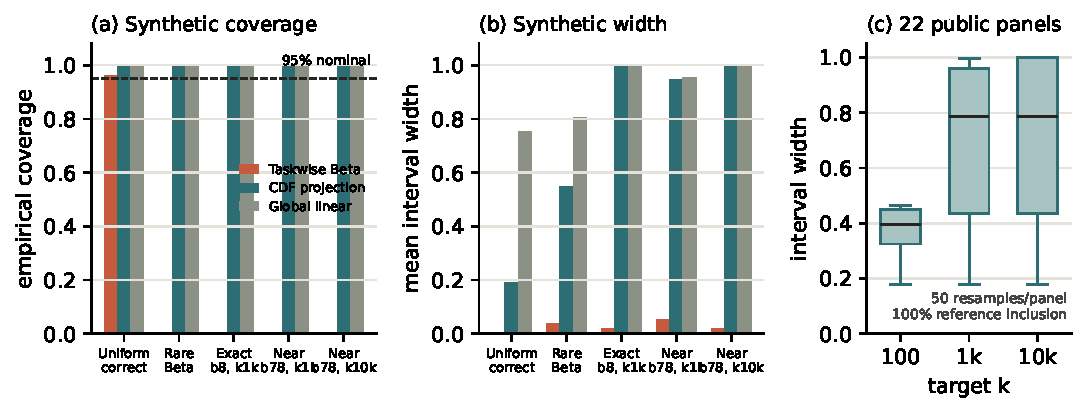
\includegraphics[width=\textwidth]{interval_audit.pdf}
\caption{Honest uncertainty adapts when the histogram is favorable and stays
wide when the data cannot distinguish the target. Panels (a) and (b) average the two sides of each exact or finite-task pair. Panel (c) shows fixed-task projection widths over 22 public panels and 50 resamples per panel. Reference inclusion is descriptive because the 10,000-response bank is finite.}
\label{fig:intervals}
\end{figure*}

Figure~\ref{fig:intervals}(a,b) shows a sharp split. The taskwise Beta interval covers \(96.25\%\) under the exact Uniform model, with mean width \(0.0059\). It has zero coverage under every other law. Its mean widths remain between \(0.0198\) and \(0.0550\) on the adversarial pairs. Both honest procedures cover all 3,200 datasets. Projection materially adapts on benign histograms: its mean width is \(0.190\) rather than \(0.752\) under Uniform, and \(0.547\) rather than \(0.806\) under the rare Beta law. It correctly approaches width one on the indistinguishable pairs.

\paragraph{Public response-bank audit.}
We use all 22 panels released by \citet{brown2024}, covering four benchmarks and model sizes from 70M to 70B. Each panel contains 127--140 tasks and 10,000 responses per task. For each of 50 shuffles, a total budget of 10,000 is allocated equally, giving 71--78 observed attempts per task. The remaining full bank defines empirical pass@\(k\) references. We evaluate population Beta-binomial MLE \citep{kazdan2025}, direct plug-in, binomial smoothed Good--Toulmin \citep{orlitsky2016}, taskwise Beta, and our fixed-task projection interval.

\begin{table}[t]
\caption{Public audit at total budget 10,000. Point columns report MAE over
1,100 panel-resamples. The last two columns report the taskwise Beta interval coverage and projection mean width.}
\label{tab:public}
\centering
\small \setlength{\tabcolsep}{3.0pt}
\begin{tabular}{rrrrrr}
\toprule
\(k\) & Pop.\ B. & SGT & Task B. & TB cov. & Proj.\ width\\
\midrule
100    & .018 & .016 & .290 & .090 & .371\\
1,000  & .041 & .200 & .384 & .089 & .714\\
10,000 & .070 & .353 & .333 & .091 & .721\\
\bottomrule
\end{tabular}
\end{table}

Table~\ref{tab:public} shows that the population Beta model is a useful point forecast on average. Its MAE nevertheless grows fourfold from pass@100 to pass@10000, and 17\% of its far-horizon forecasts err by more than 0.1. Smoothed Good--Toulmin is competitive at pass@100 but deteriorates beyond its logarithmic extrapolation regime. Taskwise Beta intervals are extremely narrow at the far target, with mean width \(0.0118\), and include the finite-bank reference only \(9.1\%\) of the time. This is not a formal coverage evaluation because the reference is noisy and reuses the bank. It does show that posterior concentration within a taskwise model is not a substitute for extrapolation robustness.

The projection interval includes every reference. Its mean width rises from \(0.371\) at pass@100 to \(0.714\) at pass@1000 and \(0.721\) at pass@10000. At the two farther targets, 40.5\% of intervals are wider than 0.9. The method is informative for favorable panels and candidly uninformative where the available attempts do not resolve rare successes.

\begin{figure*}[t]
\centering
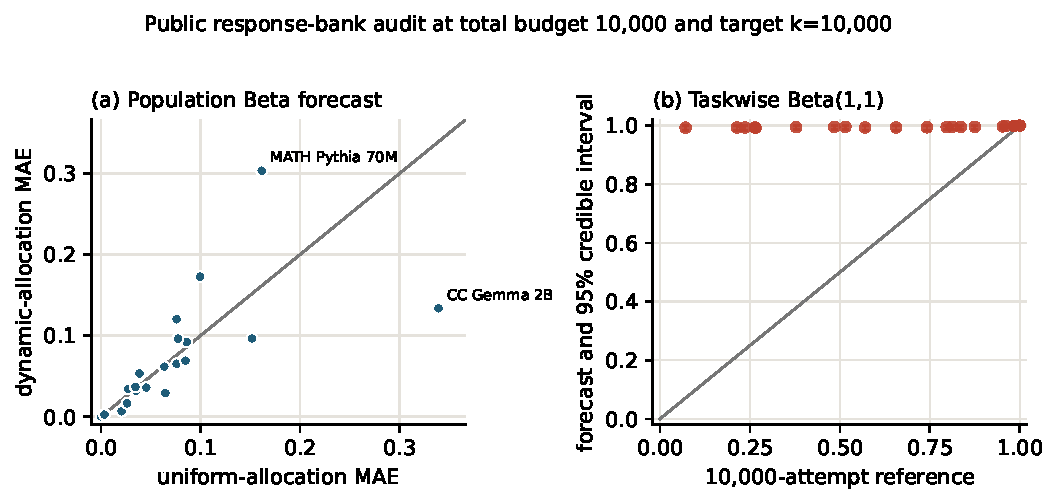
\includegraphics[width=0.86\textwidth]{real_forecast_audit.pdf}
\caption{Public response-bank forecasts at total budget 10,000 and target
\(k=10{,}000\). Left: dynamic allocation usually tracks uniform allocation rather than removing model error. Right: taskwise Beta credible intervals are much narrower than their discrepancies from the finite-bank reference.}
\label{fig:public}
\end{figure*}

Figure~\ref{fig:public} separates allocation from extrapolation. Dynamic allocation reduces mean population-Beta MAE from \(0.0697\) to \(0.0667\), only \(4.3\%\), and does not uniformly dominate equal allocation across panels. Better allocation can reduce sampling error, but Proposition \ref{prop:adaptive} shows that a per-task cap cannot resolve the underlying moment ambiguity.

\section{Related Work and Limitations}

\paragraph{Species extrapolation.}
The functional in \eqref{eq:target} is the normalized incidence-based species accumulation curve of \citet{colwell2004}. That work gives unbiased interpolation and parametric finite-mixture extrapolation. Smoothed Good--Toulmin estimators attain logarithmic extrapolation factors in abundance and Bernoulli-product incidence models \citep{orlitsky2016}. Rational continuations and parametric accumulation-rate models can work much farther \citep{daley2013,shestopaloff2025}, but the parametric bootstrap intervals of \citet{shestopaloff2025} inherit structural bias. For unbounded total richness, \citet{mao2007} prove a more severe discontinuity that permits only one-sided inference. Our bounded finite-horizon target instead has a nontrivial, exactly quantified diameter.

\paragraph{Functional estimation and partial identification.}
Polynomial approximation is a standard tool for minimax functional estimation \citep{jiao2015}. Moment projection is also classical, and our confidence-band projection is related to generic partially identified inference \citep{kaido2019}. A concurrent paper studies partial identification of latent truth from dependent LLM reports \citep{chen2026}. Its target and observation model differ from repeated-attempt success. Our contribution is the pass@\(k\)-specific diameter and horizon, the finite-task modulus, and honest constructions tied to current evaluation practice.

\paragraph{Limitations.}
The model assumes conditionally independent attempts with a stable task-specific probability. Prompt variation, correlated decoding, verifier errors, and nonstationary systems require a different observation model. \citet{zhou2026} show that deterministic activation interventions can reach some tasks missed by ordinary sampling, reinforcing that \(P\) is specific to a declared decoding regime rather than an intrinsic measure of task hardness. The Hellinger modulus values are feasible lower-bound witnesses, not certified global optima. Our public references are finite response banks, not latent truth, and the projection intervals intentionally trade width for assumption-robust coverage. Finally, favorable scientific restrictions on the lower tail of \(F\) can yield much tighter valid inference. Developing sensitivity analyses indexed by such restrictions is an important next step.

\section{Conclusion}

With \(b\) attempts per task, pass@\(k\) is a finite-moment extrapolation problem. Its sharp nonparametric ambiguity is \(2E_{b,k}\), with a transition near \(k=b^2\). Finite task sampling can make honest intervals wide even before that population boundary is reached. Parametric forecasts remain valuable when their assumptions are defensible, but narrow uncertainty beyond the observed budget is evidence about a model as well as evidence from data. Reporting that distinction makes repeated-inference scaling claims more auditable.

\section*{Reproducibility Statement}

The supplement provides complete proofs, data provenance, optimization details, and commands. The artifact contains deterministic tests, all witness laws, raw and summarized rows, and scripts that regenerate every table and figure. Public data are retrieved from the authors' released repository.

\balance
\bibliography{references}

\end{document}
